\documentclass[11pt]{article}
\usepackage{naaclhlt2012}
\usepackage{times}
\usepackage{latexsym}
\usepackage{url}
\usepackage{graphicx}
\usepackage{subfig}
\usepackage{amsmath}
\usepackage{array}
\usepackage{multirow}
\usepackage{rotating}


\author{Juri Ganitkevitch, Benjamin Van Durme \and
  Chris Callison-Burch \\
  Department of Computer Science, Johns Hopkins University \\
  Baltimore, MD 21218, USA}

\title{Monolingual Distributional Similarity for Text to Text Generation}

\begin{document}
\maketitle

\begin{abstract}
  Previous work obtained collections of paraphrases by either relying
  on sentence-aligned parallel datasets, or by using distributional
  similarity metrics over large text corpora. Our approach combines
  these two orthogonal sources of information by directly integrating
  them into the decoding algorithm. We hope to report significant
  improvements in output quality on an array of text-to-text
  generation tasks.
\end{abstract}

\section{Introduction}

A wide variety of applications in natural language processing can be
cast in terms of text-to-text generation. Given input in the form of
natural language, a text-to-text generation system produces natural
language output that fulfills previously defined constraints and
objectives on both the text's surface form and meaning. Paraphrases,
i.e.\ differing textual realizations of the same meaning, are a
crucial components of text-to-text generation systems, and have been
successfully applied to tasks such as multi-document summarization,
query expansion, question answering, sentence compression and
simplification
\cite{Barzilay1999,BarzilayThesis,mckeown:1979:ACL,Anick1999,Ravichandran2002,Riezler2007}.

Recently, \newcite{Ganitkevitch2011} presented an approach for
sentential paraphrasing derived from state-of-the-art statistical
machine translation systems. They described a large-scale extraction
method for syntactically annotated paraphrases from bilingual parallel
corpora, as well as an adaptation framework that allowed for
straight-forward, non-naive adaptation of the system to any given
sentential text-to-text generation task.

In this paper, we describe an extension of
\newcite{Ganitkevitch2011}'s approach by introducing a new component
into the paraphrasing system that is not derived from the statistical
machine translation domain and present an orthogonal source of
information: monolingual distributional similarity. More specifically,
we show that:

\begin{itemize}

\item Using monolingual distributional similarity features improves
  paraphrase quality past what we can achieve with features estimated
  from bilingual data. We demonstrate that different types of
  monolingual distributional information can be used to achieve
  differing effects such as improvements in grammaticality or word
  sense disambiguation, and discuss the trade-off between data sources
  with high-coverage versus smaller, more richly annotated corpora.

\item We define the notion of distributional similarity for paraphrase
  patterns that contain multi-word gaps. This generalizes over
  previous approaches that defined the notion for contiguous phrases
  or single-word gaps.

\item Finally, we compare the effectiveness of out method against a
  variety of baselines on an example text-to-text generation task,
  sentence compression. We show improvements in quality over both a
  purely bilingually sourced paraphrasing system and an ILP-based
  compression model.
\end{itemize}

In the following, we will give an overview of SCFG-based paraphrase
extraction (Section~\ref{sec-scfgs}) and monolingual distributional
similarity (Section~\ref{sec-mds}). Section~\ref{sec-scoring} presents
our rescoring model. We discuss the reranking results in
Section~\ref{sec-ranking}. We relate our work to prior research in
Section~\ref{sec-related-work}. Finally, Sections~\ref{sec-setup} and
\ref{sec-results} present our experimental setup and the results
obtained for the sentence compression task. We conclude in
Section~\ref{sec-conclusion}.

\section{Synchronous Context-Free Grammars}
\label{sec-scfgs}

\begin{figure}[!t]
\begin{center}
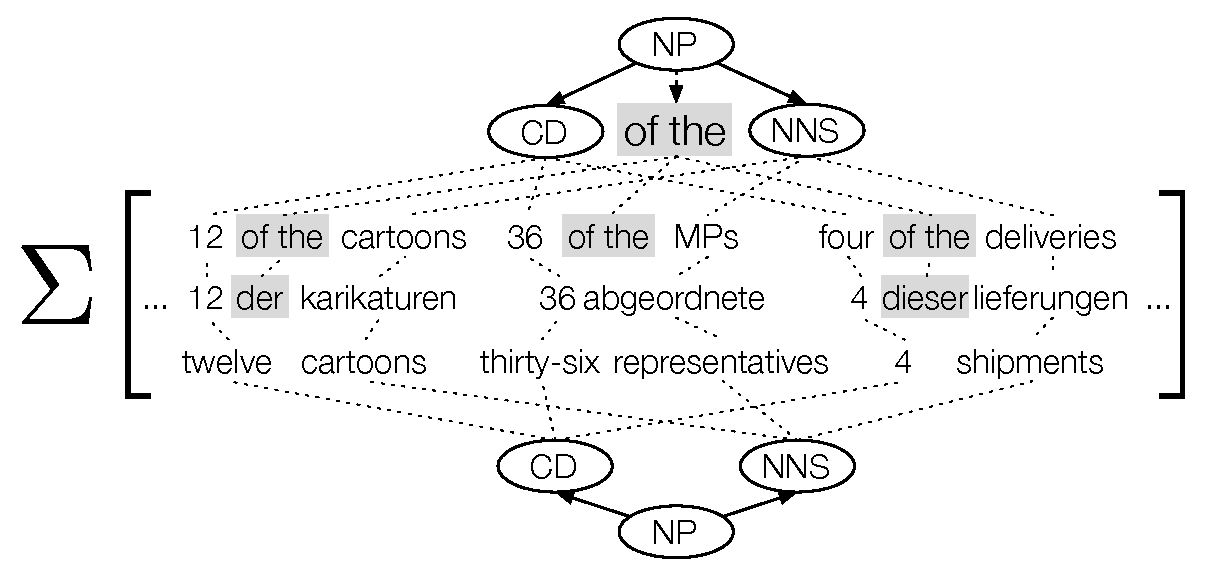
\includegraphics[width=0.99\linewidth]{figures/syntactic_pivoting.pdf}
\end{center}
\caption{An example of syntactic paraphrase extraction and feature
  estimation via the pivoting approach.}\label{fig-syntactic-pivoting}
\end{figure}

Following \newcite{Ganitkevitch2011}, we formulate our paraphrases as
a syntactically annotated \emph{ synchronous context-free grammar}
(SCFG) \cite{Aho1972,Chiang2005}.  An SCFG rule has the form:
\begin{equation*}
  \mathbf{r} = C \rightarrow \langle f, e, \sim, \vec{\varphi} \rangle ,
\end{equation*}
where the left-hand side of the rule, $C$, is a nonterminal and the
right-hand sides $f$ and $e$ are strings of terminal and nonterminal
symbols with an equal number of nonterminals. The function $\sim$
defines a one-to-one correspondency function between the nonterminals
in $f$ and $e$. Drawing on machine translation terminology, we refer
to $f$ as the \emph{source} and $e$ as the \emph{target}
side of the rule.

Each rule is annotated with a vector of feature functions
$\vec{\varphi} = \{\varphi_1 ... \varphi_N \}$ that, using a
corresponding weight vector $\vec{\lambda}$, are combined in a
log-linear model to compute the \emph{cost} of applying $\mathbf{r}$:
\begin{equation}
  \mathit{cost}(\mathbf{r}) = -\sum_{i=1}^N \lambda_i \log \varphi_i .
\end{equation}
Typical features used in the statistical machine translation models
that our system builds on are conditional phrasal, lexical and
left-hand side label probabilities, as well as a variety of count and
indicator features. We detail the feature set used in our experiments
in Section~\ref{sec-setup}.

\begin{figure}[!t]
\begin{center}
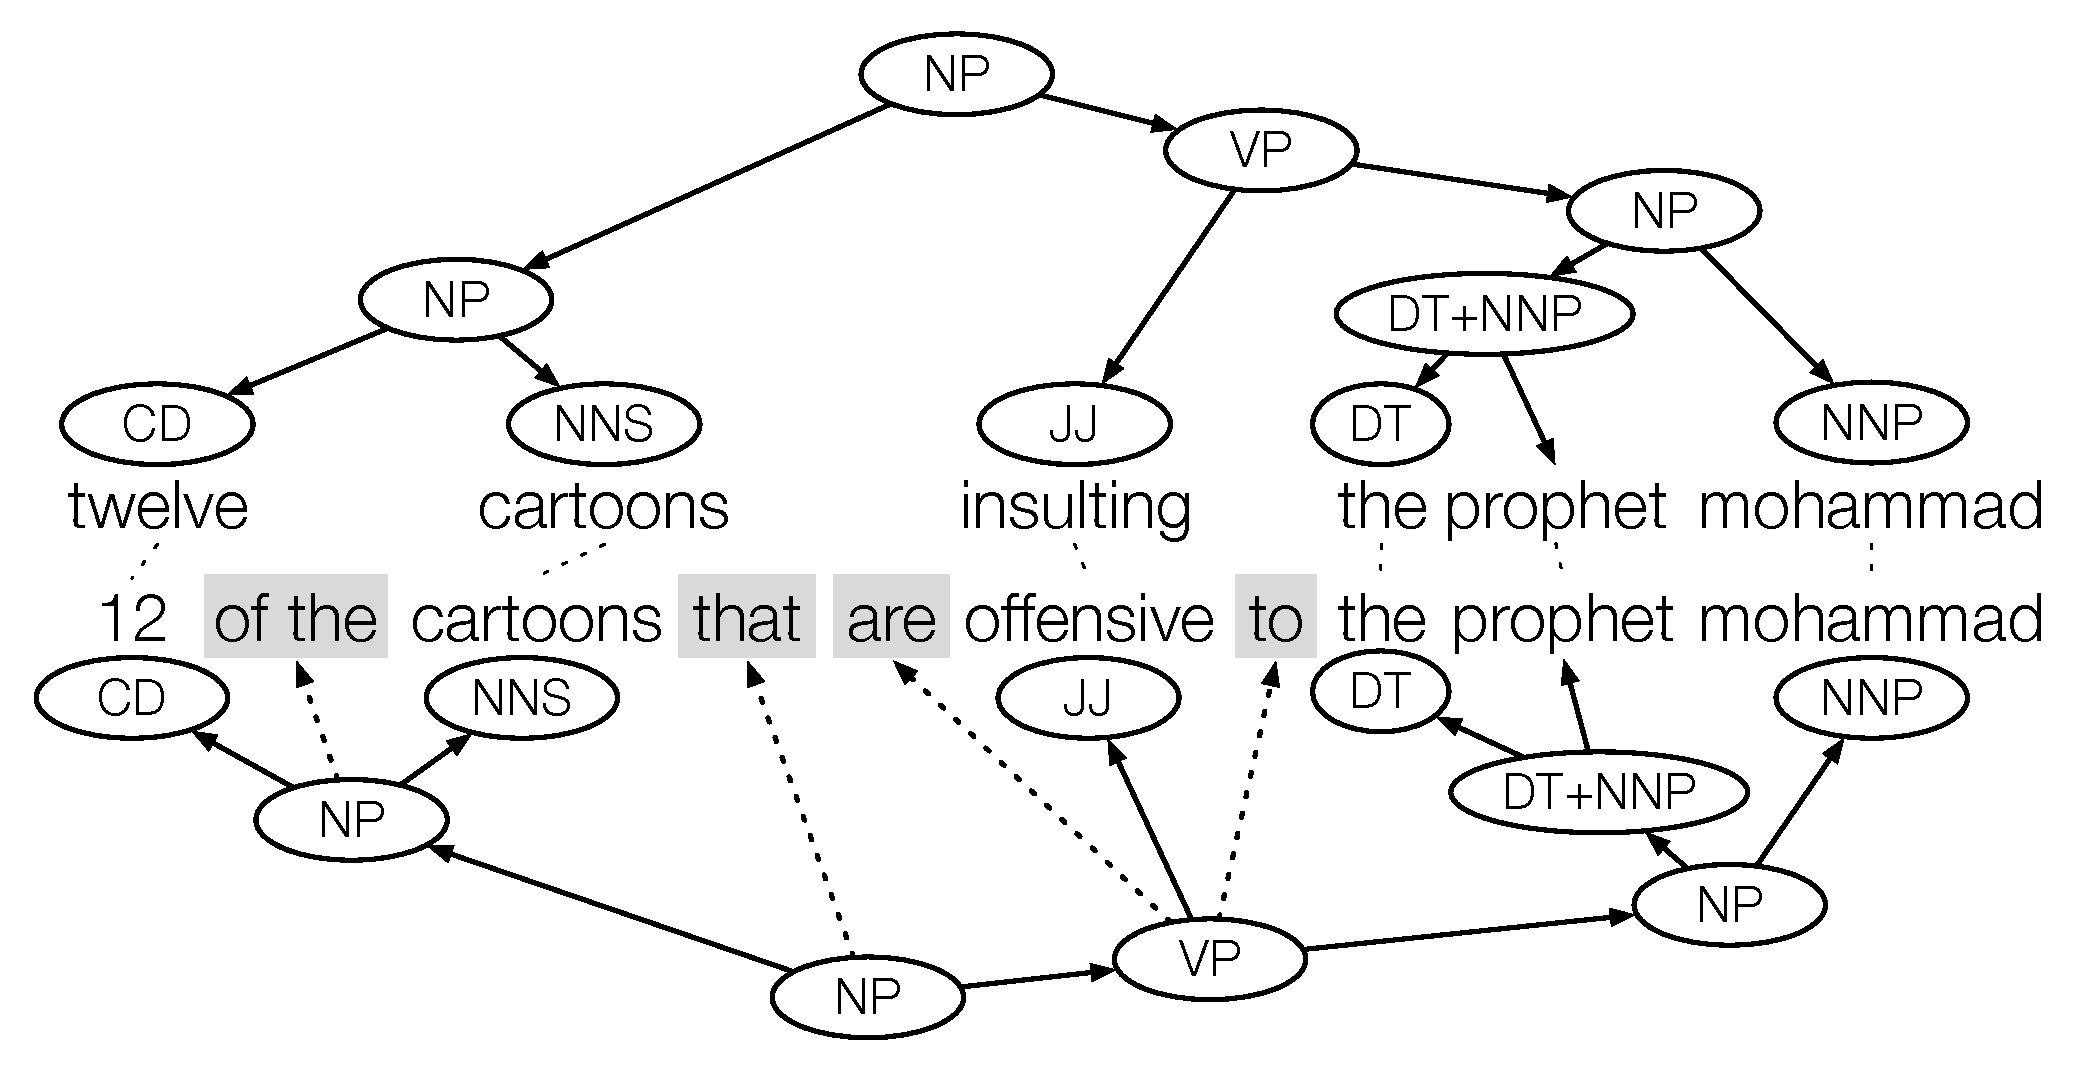
\includegraphics[width=0.99\linewidth]{figures/example_compression.pdf}
\end{center}
\caption{An example of a synchronous paraphrastic derivation.}
\label{fig-example-compression}
\end{figure}

To obtain a paraphrase grammar, we first must extract a translation
grammar that translates any given foreign language into English. Then,
for each pair of translation rules where the left-hand side $C$ and
foreign string $f$ match:
\begin{eqnarray*}
    \mathbf{r}_1 = C \rightarrow \langle f, e_1, \sim_1, \vec{\varphi}_1
  \rangle \phantom{,} \\
  \mathbf{r}_2 = C \rightarrow \langle f, e_2, \sim_2, \vec{\varphi}_2
  \rangle ,
\end{eqnarray*}
we use the intuition that two english strings $e_1$ and $e_2$ that
translate to the same foreign string $f$ are equivalent in meaning,
and \emph{pivot} over $f$ to create a paraphrase rule
\cite{Ganitkevitch2011,Callison-Burch2008,Callison-Burch2005}:
\begin{equation*}
  \mathbf{r}_p = C \rightarrow \langle e_1, e_2, \sim_p, \vec{\varphi}_p \rangle ,
\end{equation*}
with a combined nonterminal correspondency function $\sim_p$.
Similarly, the paraphrase feature vector $\vec{\varphi}_p$ is computed
from the translation feature vectors $\vec{\varphi}_1$ and
$\vec{\varphi}_2$ by following the pivoting idea. For instance, we
estimate the conditional paraphrase probability $p(e_2 | e_1)$ by
marginalizing over all shared foreign-language translations $f$:
\begin{eqnarray}
  p(e_2|e_1) &=& \sum_f p(e_2,f|e_1)\\
  &=& \sum_f p(e_2|f,e_1) p(f|e_1) \\
  &\approx& \sum_f p(e_2|f) p(f|e_1) .
\label{eq-paraphrase-probability}
\end{eqnarray}
Figure~\ref{fig-syntactic-pivoting} illustrates syntax-constrained
pivoting and feature aggregation over multiple foreign language
translations for a paraphrase pattern.
Figure~\ref{fig-example-compression} shows an example for a
synchronous paraphrastic derivation produced as a result of applying
our grammar in the decoding process.

The approach we outlined in this section relies on supervised
sentence-level parallelism to identify phrases and patterns that are
equivalent in meaning. When extracting paraphrases from monolingual
text, we have to rely on an entirely different set of semantic cues
and features.

\section{Monolingual Distributional Similarity}
\label{sec-mds}

In absence of other correspondency information, paraphrase extraction
from monolingual corpora relies on contextual features. To describe a
phrase $e$, we define a set of features that describe the context of
an occurrence of $e$ in our corpus. The resulting feature vectors
$\vec{s}_{e,i}$ are aggregated over all occurrences of $e$, resulting
in a \emph{distributional} signature for $e$, $\vec{s}_e = \sum_i
\vec{s}_{e,i}$.  Following the intuition that phrases with similar
meanings occur in similar contexts, we can then identify $e'$ as a
paraphrase of $e$ by computing the cosine similarity between their
distributional signatures:
\begin{equation*}
  \mathit{sim}(e, e') = \frac{\vec{s}_e \cdot \vec{s}_{e'}}{|\vec{s}_e||\vec{s}_{e'}|}.
\end{equation*}

The features used to describe the context of a phrase differ by
application and data source. Both \newcite{Lin2001} and
\newcite{ChurchHanks91} use a rich feature set based on constituency
and dependency parses of the text corpora they extract paraphrases
from. In their work, a phrase is described by the various syntactic
relations it has with lexical items in its context, such as the set of
verbs it appears is seen as the subject of, or the set of adjectives
that modify it. 

However, when moving to vast text collections or collapsed
representations of large text corpora, parsing can become impractical
or even impossible. In these cases using simple features based on
lexical $n$-grams has proven to be effective
\cite{LapataKellerSaLP05,Bhagat2008,LinEtAlLREC10,VanDurmeLallACL10}.

\begin{figure}[!t]
\begin{center}
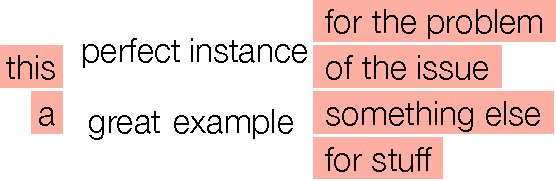
\includegraphics[width=0.99\linewidth]{figures/ngram_context.pdf}
\end{center}
\caption{An example of immediate lexical context acquisition over
  n-gram corpora.}\label{fig-ngram-context}
\end{figure}

In order to investigate the impact of the feature set used, we chose
to extract two collections of distributional similarity-based
paraphrases. Using a web-scale $n$-gram corpus
\cite{GoogleNgrams,LinEtAlLREC10}, we extract unigram features for the
words to the left and right for phrases up to a length of 4. The
features are weighed with the $n$-gram count given by the dataset. The
resulting collection comprised context vectors for the 200 million
most frequent 1- to 4-grams in the dataset.

For contrast, we use the constituency- and dependency-parsed Los
Angeles Times/Washington Post portion of the Gigaword corpus
\cite{Gigaword}. The following feature set is used to compute phrase
contexts over this dataset:
\begin{itemize}
\item Lexical and part-of-speech unigram and bigram features,
  drawn from a three-word window to the right and left of the phrase. 
\item Features based on dependencies for both links into and out of
  the phrase, labeled with the corresponding lexical item and POS. If
  the phrase is syntactically well-formed we additionally include
  lexical and POS features for its head.
\item Syntactic features for constituents governing the phrase, as
  well as for CCG-style slashed constituent labels for the phrase,
  split by governing constituent and missing constituent. 
\end{itemize}
Figure~\ref{fig-rich-context} illustrates our choice of feature
set. As a result we obtain context information for over 12 million 1-
to 4-gram phrases.

\begin{figure}[!t]
\begin{center}
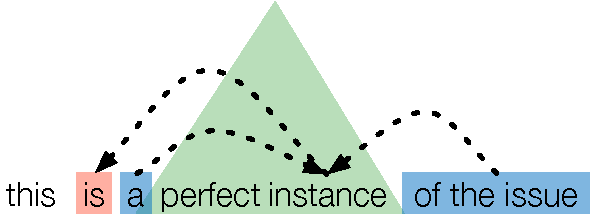
\includegraphics[width=0.99\linewidth]{figures/rich_context.pdf}
\end{center}
\caption{An example of rich monolingual distributional features over a
parsed text corpus.}\label{fig-rich-context}
\end{figure}

Much like \newcite{Ravichandran2005} and \newcite{Bhagat2008}, we
relied on Locality Sensitive Hashing (LSH), to make the use of these
large collections practical. In order to avoid explicitly computing
the feature vectors, which can be memory intensive for frequent
phrases, we chose the online LSH variant described in
\cite{VanDurmeLallACL10}. This method, based on the earlier work of
\newcite{IndykSTOC98} and \newcite{Charikar02}, approximates the
cosine similarity between two feature vectors based on the Hamming
distance in a dimensionality-reduced bitwise representation. Two
feature vectors $u$, $v$ each of dimension $d$ are first projected
through a $d \times b$ random matrix populated with draws from
$\mathcal{N}(0,1)$. We then convert the resulting $b$-dimensional
vectors into bit-vectors by setting each bit of the signature
conditioned on whether the corresponding projected value is less than
0. Now, given the bit signatures $h(\vec{u})$ and $h(\vec{v})$, we
approximate the cosine similarity of $u$ and $v$ as:
\begin{equation*}
  \mathit{sim'}(u, v) =
  \cos\Big(\frac{D(h(\vec{u}),h(\vec{v}))}{b}\pi\Big) ,
\end{equation*}
where $D()$ is the Hamming distance.



\section{Incorporating Distributional Similarity}
\label{sec-scoring}

In order for us to make the distributional similarity information
accessible to the paraphrasing system, we need to calculate similarity
scores for the paraphrastic SCFG rules in our grammar. However, the
similarity information we obtain from our monolingual sources is
defined for lexical $n$-grams only, not for patterns with gaps in
them.  

We close this gap, by decomposing the discontinuous patterns that make
up the right-hand sides of a rule $\mathbf{r}$ into pairs of
contiguous phrases $P(\mathbf{r}) = (\bar{e}, \bar{e}')$, for which we
can look up distributional signatures and compute similarity
scores. This decomposition into phrases is non-trivial, since our
sentential paraphrase rules often involve significant reordering or
structural changes. To avoid comparing unrelated phrase pairs, we
require $P(\mathbf{r})$ to be consistent with a token alignment
$\mathbf{a}$. We define and compute $\mathbf{a}$ analogously to the
word alignments used in statistical machine
translation. Figure~\ref{fig-pattern-scoring} shows an aligned rule
and the phrase pairs we extract from it.

\begin{figure}[!t]
\begin{center}
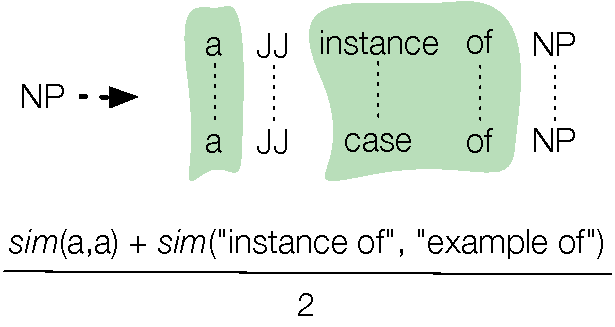
\includegraphics[width=0.70\linewidth]{figures/pattern_scoring.pdf}
\end{center}
\caption{Scoring a rule by extracting and scoring contiguous phrases
  consistent with the alignment.}\label{fig-pattern-scoring}
\end{figure}

We define the overall similarity score of the rule to be the average
of the similarity scores of all extracted phrase pairs:
\begin{equation*}
  \mathit{sim}(\mathbf{r}, \mathbf{a}) = \frac{1}{|P(\mathbf{a})|}
  \sum_{(e, e') \in P(\mathbf{a})}\mathit{sim}(e, e') .
\end{equation*}
This is done to achieve a sparsity-reducing effect similar to backing
off in statistical $n$-gram language models. Since the distributional
signatures for long, rare phrases may be computed from only a handful
of occurrences, we additionally query for the shorter sub-phrases that
are more likely to have been observed often enough for reliable
signature and thus similarity estimates.

Our two similarity scores are incorporated into the paraphraser as an
additional rule feature $\varphi_{\mathit{sim}}$. The corresponding
weight $\lambda_{\mathit{sim}}$ is estimated along with the other
$\lambda_i$ in our training framework, detailed in
Section~\ref{sec-setup}.


\section{Paraphrase Ranking}
\label{sec-ranking}

Properly estimating the quality of a paraphrase pair is crucial to a
paraphrase system's usefulness to text-to-text applications. 

Pivoted paraphrases and ones based on monolingual distributional
similarity are drawing on orthogonal sources of information, and we
believe that combining the two will improve paraphrase quality beyond
either individual approach.

We test our hypothesis in two ways: applying the distributional
similarity-annotated paraphrase system to a text-to-text task (see
Section~\ref{sec-results}), and by examining the effect the
incorporation of distributional similarity has on the ranking of
paraphrases within our grammar.

We also compare the two types of distributional similarity at hand:
simple lexical features estimated collected from a large-scale
$n$-gram corpus, against a richer feature set but with significantly
less coverage.

\begin{table*}[t]
\small
\begin{center}
\begin{tabular}{|cl|cl|cl|cl|}
  \hline
  \multicolumn{8}{|c|}{phrase!} \\
  \hline
  baseline 1 & 0.96 &
  ngrams 1 & 0.9 &
  rich 1 & 0.96 &
  combined 1 & 0.9 \\

  baseline 2 & 0.96 &
  ngrams 2 & 0.9 &
  rich 2 & 0.96 &
  combined 2 & 0.9 \\

  baseline 3 & 0.96 &
  ngrams 3 & 0.9 &
  rich 3 & 0.96 &
  combined 3 & 0.9 \\


  baseline 4 & 0.96 &
  ngrams 4 & 0.9 &
  rich 4 & 0.96 &
  combined 4 & 0.9 \\


  baseline 5 & 0.96 &
  ngrams 5 & 0.9 &
  rich 5 & 0.96 &
  combined 5 & 0.9 \\

  \hline
  \multicolumn{8}{c}{} \\
  \hline
  \multicolumn{8}{|c|}{different phrase!} \\
  \hline
  baseline 1 & 0.96 &
  ngrams 1 & 0.9 &
  rich 1 & 0.96 &
  combined 1 & 0.9 \\

  baseline 2 & 0.96 &
  ngrams 2 & 0.9 &
  rich 2 & 0.96 &
  combined 2 & 0.9 \\

  baseline 3 & 0.96 &
  ngrams 3 & 0.9 &
  rich 3 & 0.96 &
  combined 3 & 0.9 \\


  baseline 4 & 0.96 &
  ngrams 4 & 0.9 &
  rich 4 & 0.96 &
  combined 4 & 0.9 \\


  baseline 5 & 0.96 &
  ngrams 5 & 0.9 &
  rich 5 & 0.96 &
  combined 5 & 0.9 \\

  \hline
\end{tabular}
\end{center}
\normalsize
\caption{Comparison of paraphrase rankings for }
\label{grammar_stats}
\end{table*}



\section{Experiments}
\label{sec-results}

\subsection{Sentence Compression}

To evaluate our method on a real text-to-text application, we chose to
adopt the setting and datasets from \cite{Ganitkevitch2011}. We train
our paraphrasing system to produce sentence level compression by way
of sentential paraphrasing. We contrast our distributional
similarity-informed paraphrase system with an uninformed pivoting-only
(but otherwise identical) baseline, as well as an implementation of
\newcite{Clarke2008}'s state-of-the-art compression model which uses a
series of constraints in an integer linear programming (ILP) solver.

\subsection{Experimental Setup}
\label{sec-setup}

\begin{table}
\small
\begin{center}
\begin{tabular}{|c|r|}
  \hline
  Grammar & \multicolumn{1}{c|}{\# Rules} \\
  \hline
  total & 42,353,318 \\
  w/o identity & 23,641,016 \\
  w/o complex constituents & 6,439,923 \\
  w/o complex const.\ \& identity & 5,097,250 \\
  \hline
\end{tabular}
\end{center}
\normalsize
\caption{Number and distribution of rules in our paraphrase
  grammar. Note the significant number of identity paraphrases and
  rules with complex nonterminal labels.}
\label{grammar_stats}
\end{table}

We extracted our paraphrase grammar from the French--English portion
of the Europarl corpus (version 5). The Berkeley aligner and the
Berkeley parser were used to align the bitext and parse the English
side, respectively. The paraphrase grammar was produced using the
Hadoop-based Thrax grammar extractor's paraphrase mode. The syntactic
nonterminal labels we allowed in the grammar were limited to
constituent labels and CCG-style slashed categories. Paraphrase
grammars extracted via pivoting tend to grow very large. To keep the
grammar size manageable, we pruned away all paraphrase rules whose
phrasal paraphrase probabilities $p(e_1|e_2)$ or $p(e_2|e_1)$ were
smaller than $0.001$.

We extended the feature set used by \newcite{Ganitkevitch2011} with a
number of features that aim to better describe a rule's compressive
power: on top of the word count features $c_{\mathit{src}}$ and
$c_{\mathit{tgt}}$ and the word count difference feature
$c_{\mathit{diff}}$, we add character based count and difference
features $\mathit{char}_{\mathit{src}}$,
$\mathit{char}_{\mathit{tgt}}$, and $\mathit{char}_{\mathit{diff}}$,
as well as log-compression ratio features $c_{\mathit{cr}} = \log
\frac{c_{\mathit{tgt}}}{c_{\mathit{src}}}$ and the analogously defined
$\mathit{char}_{\mathit{cr}}$.

For model tuning and decoding, we used the Joshua machine translation
system \cite{Joshua-3.0}. The model weights were estimated using an
implementation of the PRO tuning algorithm \cite{PRO2011}, with
\textsc{Pr\'ecis} as our objective function \cite{Ganitkevitch2011}.  The
language model used in our paraphraser and the \newcite{Clarke2008}
baseline system is a Kneser-Ney discounted 5-gram model estimated on
the Gigaword corpus using the SRILM toolkit \cite{SRILM}.

\subsection{Evaluation Results}

To rate the quality of our output, we solicit human judgments of the
compressions along two five-point scales: grammaticality and
meaning. Judges are instructed to decide how much the meaning from a
reference translation is retained in the compressed sentence, with a
score of 5 indicating that all of the important information is
present, and 1 being that the compression does not retain any of the
original meaning. Similarly, a grammar score of 5 indicates perfect
grammaticality, and a grammar score of 1 is assigned to sentences that
are entirely ungrammatical. It is known that evaluation quality
correlates linearly with compression rate \cite{Napoles2011}. Thus, to
ensure fairness in comparing our systems, we adjust compression rates
to closely match on the sentence-level.

In Table~\ref{human_judgments} we compare our distributional
similarity-augmented paraphraser to the plain pivoting baseline and
the ILP approach at a compression rate of $\approx 0.75$. We can see
that the paraphrase approach significantly outperforms ILP on meaning
retention. However it shows notable weaknesses in
grammaticality. Adding $n$-gram-based distributional similarity
information to the paraphrases not only recovers most of the
difference in grammaticality, but also yields an additional gain in
the compressions' meaning retention.

Table~\ref{test_examples} shows an example sentence drawn from our
test set and the compressions produced by the different systems. We
see that both the paraphrase and ILP systems produce good quality
results, with the paraphrase system retaining the meaning of the
source sentence more accurately.

 \begin{table}
   \small
   \begin{center}
     \begin{tabular}{|c|c|c|c|}
       \hline
       & CR & Meaning & Grammar \\
       \hline
       Reference & 0.80 &  4.80 & 4.54 \\
       \hline
       ILP & 0.74 & 3.44 & {\bf 3.41} \\
       \hline
       \hline
       PC & 0.78 & 3.53 & 2.98 \\
       \hline
       PC + $n$-gram & 0.80 & 3.65 & 3.16 \\
       PC  + rich features & 0.79 & {\bf 3.70} & 3.26 \\
       \hline
       \hline
       Random Deletions & 0.78 & 2.91 & 2.53 \\
       \hline
     \end{tabular}
   \end{center}
   \normalsize
   \caption{Results of the human evaluation on longer compressions:
     pairwise compression rates (CR), meaning and grammaticality scores. 
     Bold indicates a statistically significance difference at $p <
     0.05$.}
   \label{human_judgments}
 \end{table}


\begin{table*}[!th]
\begin{center}
\small
{
\renewcommand{\arraystretch}{1.5}
\begin{tabular}{|c|>{\raggedright}m{13.2cm}|}
%  \hline
%  & \multicolumn{1}{|c|}{Sentences}  \\
  \hline

  Source & should these political developments have an impact on sports
  ? \tabularnewline
  \hline
  Reference & should these political events affect sports ? \tabularnewline
  \hline
  Rich & should these events have an impact on sports ? \tabularnewline
  \hline
  $n$-gram & these political developments impact on sports ? \tabularnewline
  \hline
  PC & should these events impact on sports ? \tabularnewline
  \hline
  ILP & political developments have an impact \tabularnewline
  \hline
  \hline

  Source & now we have to think and make a decision about our direction
  and choose only one way . thanks . \tabularnewline
  \hline
  Reference & we should ponder it and decide our path and follow it , thanks
  . \tabularnewline
  \hline
  Rich & now we think and decide on our way and choose one way . thanks
  . \tabularnewline
  \hline
  $n$-gram & now we have and decide on our way and choose one way . thanks
  . \tabularnewline
  \hline
  PC & now we have and decide on our way and choose one way . thanks
  . \tabularnewline
  \hline
  ILP &  we have to think and make a decision and choose way thanks
  \tabularnewline
  \hline
  \hline

  Source &  we are not poor . in fact , in our country , we are rich , and
  our poverty is in the lack of patriotism by some of the officials
  among us . \tabularnewline
  \hline
  Reference &  we are not poor in our country ; we are rich . our poverty is
  in the lack of patriotism of some of our officials . \tabularnewline
  \hline
  Rich & we are not poor . in fact in our country we are rich , and our
  poverty is the lack of patriotism by some officials us
  . \tabularnewline
  \hline
  $n$-gram & we are poor . in fact , our country , we are rich and
  poverty is no patriotism by some officials us . \tabularnewline
  \hline
  PC & we are not poor . in fact , in our country rich , and poverty
  is no patriotism by some officials among us . \tabularnewline
  \hline
  ILP & we are not poor in fact in our country we are rich and our
  poverty is in lack by some of officials among us \tabularnewline
  \hline
\end{tabular}
}
\normalsize
\end{center}
\caption{Example compressions produced by the two systems in
  Table~\ref{human_judgments} for three input sentences from our test
  data.}
\label{test_examples}
\end{table*}

\section{Conclusion}
\label{sec-conclusion}

We presented a method to incorporate monolingual distributional
similarity into linguistically informed sentential paraphrase
extracted from bilingual parallel data. We investigate both the effect
of varying the feature set used for determining the distributional
signatures of phrases and show that TODO. Additionally, we evaluate
our integrated paraphrases on a text-to-text generation task and show
that our method improves over both a strong paraphrastic baseline and
a specialized state-of-the-art system.

\bibliographystyle{naaclhlt2012}
\bibliography{monods_t2t}
\end{document}